\documentclass[mathserif
%, handout
]{beamer}
 
  \useoutertheme{wuerzburg}
  \useinnertheme[outline]{chamfered}
 \usecolortheme{shark}
 \definecolor{MyBackground}{RGB}{243,246,249}
 \setbeamercolor{background canvas}{bg=MyBackground}

 %\usecolortheme[snowy]{owl}
 %\usecolortheme{owl}
 
 %\usetheme{Warsaw}
 %\usecolortheme{spruce}

\usepackage{tabu}
\usepackage{rotating}
\usepackage[]{algorithm2e}
\usepackage{color, colortbl}
%\usepackage{default}
\usepackage{fontspec}
\usepackage{polyglossia} 
\setmainlanguage{vietnamese}
%\setdefaultlanguage{vietnamese} 
%\setmainfont{Palatino}
 \usepackage{wasysym}
\usepackage{pifont}% http://ctan.org/pkg/pifont

\usepackage{multicol}
\usepackage{sidecap}

\usepackage{hyperref}

\usepackage{pgf}    
\usepackage{tikz}
\usetikzlibrary{arrows,automata,decorations.pathmorphing,backgrounds,positioning,fit}
\usepackage{array}
\usepackage{listings}

\usepackage{enumerate}
%\usepackage{amsmath,mathtools}
%		\usepackage{fink}

\usepackage{amsmath,amsthm, amssymb}
\usepackage{microtype}
\usetikzlibrary{arrows,automata}
\usetikzlibrary{decorations.pathmorphing}


\usetikzlibrary{calc}

 

\usetikzlibrary{trees}
\usepackage{listings}

\setbeamertemplate{footline}[frame number]
\setbeamertemplate{navigation symbols}{}%remove navigation symbols

%\usepackage{listingsutf8}

%\setbeameroption{show notes on second screen=right}


  
%\newtheorem{Lemme}{Bổ đề} 
%\newtheorem*{LI}{Lemme d'itération infinie}

%\newtheorem{Proposition}{Mệnh đề}[section]
%\newtheorem{Theorem}{Định lý}[section]
%\newtheorem{Corollaire}{Hệ quả}[section]
%\newtheorem*{Conjecture}{Giả thuyết}
% \newtheorem*{Probleme}{Bài toán}
% \newtheorem*{Fait}{Fait}
% 
% 
% \theoremstyle{definition} \newtheorem{Definition}{Định nghĩa}
% \theoremstyle{definition} \newtheorem{example}{Ví dụ}
% \theoremstyle{remark} \newtheorem*{Remarque}{Chú ý}


\usetikzlibrary{arrows,automata}



\usetikzlibrary{trees}


% \newcommand{\mnvect}[2]
% {
%   \begin{bmatrix}	#1\\#2
%   \end{bmatrix}
% }

\definecolor{olive}{rgb}{0.3, 0.4, .1}
\definecolor{fore}{RGB}{249,242,215}
\definecolor{back}{RGB}{51,51,51}
\definecolor{title}{RGB}{255,0,90}
\definecolor{dgreen}{rgb}{0.,0.7,0. }
\definecolor{gold}{rgb}{1.,0.84,0.}
\definecolor{JungleGreen}{cmyk}{0.99,0,0.52,0}
\definecolor{BlueGreen}{cmyk}{0.85,0,0.37,0}
\definecolor{RawSienna}{cmyk}{0,0.72,1,0.45}
\definecolor{Magenta}{cmyk}{0,1,0,0} 



%

%\setlength{\topmargin}{0cm} \setlength{\oddsidemargin}{0cm}
%\setlength{\evensidemargin}{0cm} \setlength{\textwidth}{17truecm}
%\setlength{\textheight}{21.0truecm}


%\parindent = 3 pt
%\parskip = 12 pt

%\newtheorem*{LI}{Lemme d'itération infinie}



\newtheorem{prprt}{Propriété}
\newtheorem{prpstn}{Mệnh đề}
\newtheorem{thrm}{Định lý}
\newtheorem{lmm}{Bổ đề}

\newtheorem{crllr}{Hệ quả}
\newtheorem{clm}{Fait}
\newtheorem{nt}{Notation}
 
\newtheorem*{cnjctr}{Conjecture}
\newtheorem{prblm}{Problème}
\newtheorem{qstn}{Question}
\newtheorem{fct}{Fait}
%\newtheorem{xmpl}{Exemple}
\newtheorem{rmrk}{Nhận xét}

\theoremstyle{example}
\newtheorem{xmpl}{Ví dụ}
\newtheorem{xrcs}{Bài tập}
  \newtheorem{dfntn}{Định nghĩa}
  

% \declaretheorem[name=Problème]{prblm}
% \declaretheorem[name=Question, style=remark, numbered=no]{qstn}

% \declaretheorem[name=Théorème, numberwithin=section]{thrm}
% \declaretheorem[name=Lemme, sibling=thrm]{lmm}
% \declaretheorem[ name=Propriété, sibling=thrm]{prprt}
% \declaretheorem[ name=Proposition, sibling=thrm]{prpstn}
% \declaretheorem[name=Corollaire, sibling=thrm]{crllr}
% \declaretheorem[name=Fait, sibling=thrm]{fct}
% \declaretheorem[name=Notation, sibling=thrm]{nt}


% \declaretheorem[style=definition, name=Définition, sibling=thrm]{dfntn}

% %\theoremstyle{definition} \newtheorem{dfntn}{Définition}[section]

% \renewcommand\thmcontinues[1]{reprise de p.\,\pageref{#1}}

% \declaretheorem[style=remark, name=Exemple%, numberwithin=section
% ]{xmpl}

% \declaretheorem[style=remark, name=Remarque, numbered=no]{rmrk}

% %\declaretheorem[style=definition,numberwithin=chapter,name = Exemple]{xmpl}

% %\theoremstyle{remark} \newtheorem{xmpl}{Exemple}[chapter]

% %\theoremstyle{remark} \newtheorem*{rmrk}{Remarque}



\newtheorem{cs}{Cas}


\def\mclose{\texttt{close}}
\def\mopen{\texttt{open}}

\def\mmclose{\texttt{\scriptsize close}}
\def\mmopen{\texttt{\scriptsize open}}



% \newcommand{\mvect}[2]
% {
% \bigl[ \begin{smallmatrix}
% #1\\ #2
% \end{smallmatrix} \bigr]
% }

% \newcommand{\mnvect}[2]
% {
%   \begin{bmatrix}	#1\\#2
%   \end{bmatrix}
% }

% % \newcommand{\mnvect}[2]
% % {
% % #1/#2
% %   % \begin{bmatrix}	#1\\#2
% %   % \end{bmatrix}
% % }

% \newcommand{\XMPL}[3]
% {
%   \begin{xmpl}
%     Soient $L=\{#1\}$ et $\Sigma=\{#2\}$. On peut vérifier que $L$ est \orl\ avec le
%     relateur de base $#3$.
%   \end{xmpl}
% }

% \newcommand{\XMP}[4]
% {
%   \begin{xmpl}[#4]
%     Soient $L=\{#1\}$ et $\Sigma=\{#2\}$. On peut vérifier que $L$ est \orl\ avec le
%     relateur de base $#3$.
%   \end{xmpl}
% }

% \newcommand{\Pui}[2]
% {
%   #1^{\leq #2}
% }


% % \newcommand{\XMPL1}[4]
% % {
% %   \begin{xmpl}
% %     Soient $L=\{#1\}$ et $\Sigma=\{#2\}$. Il est clair que $L$ est \orl\ avec le
% %     relateur de base $#3$. $L^\omega$ est un 
% %   \end{xmpl}
% % }

% \def\vvs{\vspace{11pt}}
% \def\nni{\noindent}


% \newcommand{\cas}[1]
% {
% \vvs\nni
% \textbf{Cas #1 :}
% }



% \newcommand{\souscas}[1]
% {
% \vvs\nni
% \textbf{Sous-cas #1 :}
% }

% \def\pcom{paire de mots incompatibles}
% \def\wpcom{paire de mots $\infty$-incompatible}

% \def\upcom{une paire de mots incompatibles}
% \def\uwpcom{une paire de mots $\infty$-incompatibles}
% \def\comp{\asymp}

% \def\wg{code générateur}

%  \def\gc{code générateur}

% \def\gcx{codes générateurs}
% \def\Gcx{Codes générateurs }
% \def\ugc{un code générateur}
% \def\Ugc{un Code générateur}

% \def\wgc{$\omega$-code générateur}
% \def\wgcx{$\omega$-codes générateurs}
% \def\wGcx{$\omega$-Codes générateurs }
% \def\wugc{un $\omega$-code générateur}
% \def\wUgc{un $\omega$-code générateur}

% \def\orl {langage à un relateur}

% \def\orlx {langages à un relateur}
% \def\Orlx {Langages à un relateur}
% \def\uorl {un langage à un relateur}


% \def\ugc{un code générateur}

% \def\cp{code préfixe}

% \def\iff{si et seulement si} 
% \def\w{\omega}

% \def\CODE{la proposition~\ref{c3prop23}, $L^\omega$ n'a pas de \gc}
% \def\NOCODE{$L^\omega$ n'a pas de \gc}


\def\vs{}
\def\ni{}





%\setlength{\topmargin}{0cm} \setlength{\oddsidemargin}{0cm}
%\setlength{\evensidemargin}{0cm} \setlength{\textwidth}{17truecm}
%\setlength{\textheight}{21.0truecm}


%\parindent = 3 pt
%\parskip = 12 pt

%\newtheorem*{LI}{Lemme d'itération infinie}



\newtheorem{prprt}{Propriété}
\newtheorem{prpstn}{Mệnh đề}
\newtheorem{thrm}{Định lý}
\newtheorem{lmm}{Bổ đề}
\newtheorem{rl}{Luật}

\newtheorem{crllr}{Hệ quả}
\newtheorem{clm}{Khẳng định}
\newtheorem{nt}{Notation}
 
\newtheorem*{cnjctr}{Giả thuyết}

\newtheorem{fct}{Fait}
%\newtheorem{xmpl}{Exemple}

\theoremstyle{example}
\newtheorem{xmpl}{Ví dụ}
\newtheorem{xrcs}{Bài tập}
  \newtheorem{dfntn}{Định nghĩa}
  \newtheorem{qstn}{Câu hỏi}
\newtheorem{prblm}{Bài toán}  
   \newtheorem{sol}{Lời giải}
\newtheorem{rmrk}{Nhận xét}
  
%  \newtheorem{rmrk}{Định nghĩa}
  

% \declaretheorem[name=Problème]{prblm}
% \declaretheorem[name=Question, style=remark, numbered=no]{qstn}

% \declaretheorem[name=Théorème, numberwithin=section]{thrm}
% \declaretheorem[name=Lemme, sibling=thrm]{lmm}
% \declaretheorem[ name=Propriété, sibling=thrm]{prprt}
% \declaretheorem[ name=Proposition, sibling=thrm]{prpstn}
% \declaretheorem[name=Corollaire, sibling=thrm]{crllr}
% \declaretheorem[name=Fait, sibling=thrm]{fct}
% \declaretheorem[name=Notation, sibling=thrm]{nt}


% \declaretheorem[style=definition, name=Définition, sibling=thrm]{dfntn}

% %\theoremstyle{definition} \newtheorem{dfntn}{Définition}[section]

% \renewcommand\thmcontinues[1]{reprise de p.\,\pageref{#1}}

% \declaretheorem[style=remark, name=Exemple%, numberwithin=section
% ]{xmpl}

% \declaretheorem[style=remark, name=Remarque, numbered=no]{rmrk}

% %\declaretheorem[style=definition,numberwithin=chapter,name = Exemple]{xmpl}

% %\theoremstyle{remark} \newtheorem{xmpl}{Exemple}[chapter]

% %\theoremstyle{remark} \newtheorem*{rmrk}{Remarque}



\newtheorem{cs}{Cas}


\def\mclose{\texttt{close}}
\def\mopen{\texttt{open}}

\def\mmclose{\texttt{\scriptsize close}}
\def\mmopen{\texttt{\scriptsize open}}



% \newcommand{\mvect}[2]
% {
% \bigl[ \begin{smallmatrix}
% #1\\ #2
% \end{smallmatrix} \bigr]
% }

% \newcommand{\mnvect}[2]
% {
%   \begin{bmatrix}	#1\\#2
%   \end{bmatrix}
% }

% % \newcommand{\mnvect}[2]
% % {
% % #1/#2
% %   % \begin{bmatrix}	#1\\#2
% %   % \end{bmatrix}
% % }

% \newcommand{\XMPL}[3]
% {
%   \begin{xmpl}
%     Soient $L=\{#1\}$ et $\Sigma=\{#2\}$. On peut vérifier que $L$ est \orl\ avec le
%     relateur de base $#3$.
%   \end{xmpl}
% }

% \newcommand{\XMP}[4]
% {
%   \begin{xmpl}[#4]
%     Soient $L=\{#1\}$ et $\Sigma=\{#2\}$. On peut vérifier que $L$ est \orl\ avec le
%     relateur de base $#3$.
%   \end{xmpl}
% }

% \newcommand{\Pui}[2]
% {
%   #1^{\leq #2}
% }


% % \newcommand{\XMPL1}[4]
% % {
% %   \begin{xmpl}
% %     Soient $L=\{#1\}$ et $\Sigma=\{#2\}$. Il est clair que $L$ est \orl\ avec le
% %     relateur de base $#3$. $L^\omega$ est un 
% %   \end{xmpl}
% % }

% \def\vvs{\vspace{11pt}}
% \def\nni{\noindent}


% \newcommand{\cas}[1]
% {
% \vvs\nni
% \textbf{Cas #1 :}
% }



% \newcommand{\souscas}[1]
% {
% \vvs\nni
% \textbf{Sous-cas #1 :}
% }

% \def\pcom{paire de mots incompatibles}
% \def\wpcom{paire de mots $\infty$-incompatible}

% \def\upcom{une paire de mots incompatibles}
% \def\uwpcom{une paire de mots $\infty$-incompatibles}
% \def\comp{\asymp}

% \def\wg{code générateur}

%  \def\gc{code générateur}

% \def\gcx{codes générateurs}
% \def\Gcx{Codes générateurs }
% \def\ugc{un code générateur}
% \def\Ugc{un Code générateur}

% \def\wgc{$\omega$-code générateur}
% \def\wgcx{$\omega$-codes générateurs}
% \def\wGcx{$\omega$-Codes générateurs }
% \def\wugc{un $\omega$-code générateur}
% \def\wUgc{un $\omega$-code générateur}

% \def\orl {langage à un relateur}

% \def\orlx {langages à un relateur}
% \def\Orlx {Langages à un relateur}
% \def\uorl {un langage à un relateur}


% \def\ugc{un code générateur}

% \def\cp{code préfixe}

% \def\iff{si et seulement si} 
% \def\w{\omega}

% \def\CODE{la proposition~\ref{c3prop23}, $L^\omega$ n'a pas de \gc}
% \def\NOCODE{$L^\omega$ n'a pas de \gc}


\def\vs{}
\def\ni{}


\def\trail{hành trình đơn}
\def\Trail{Hành trình đơn}

\def\ctrail{\trail\ đóng}
\def\Ctrail{\Trail\ đóng }

\def\walk{hành trình}
\def\Walk{Hành trình}

\def\cwalk{hành trình đóng}
\def\Cwalk{Hành trình đóng}

\def\path{đường đi}
\def\Path{Đường đi}
 
\def\conn{liên thông}
\def\Conn{Liên thông}

\def\Comp{Thành phần liên thông}
\def\comp{thành phần liên thông}

\def\Cuted{Cạnh cắt}
\def\cuted{cạnh cắt}

\def\Cutve{Đỉnh cắt}
\def\cutve{đỉnh cắt}

\def\Induced{Đồ thị con cảm sinh}
\def\induced{đồ thị con cảm sinh}

 
\def\iff{{\color{blue} nếu và chỉ nếu}}

\def\ideg{\text{indeg}}
\def\odeg{\text{outdeg}}

\def\pr{\mathrm{Pr}}
\def\ex{\mathrm{Ex}}
\def\S{\mathcal{S}}
\def\var{\mathrm{Var}}

\def\F{\mathbb{F}}
\def\Z{\mathbb{Z}}
\def\N{\mathbb{N}}
\def\ord{\mathrm{ord}}
\newcommand{\bigO}{\ensuremath{\mathcal{O}}}% big-O notation/symbol


 \newcommand{\defi}[1]{{\color{blue}{\textbf{\emph{#1}}}}}
\newcommand{\contradiction}{{\hbox{%
    \setbox0=\hbox{$\mkern-3mu\times\mkern-3mu$}%
    \setbox1=\hbox to0pt{\hss$\times$\hss}%
    \copy0\raisebox{0.5\wd0}{\copy1}\raisebox{-0.5\wd0}{\box1}\box0
}}}

\newcommand{\cmark}{{\color{blue}\Large\ding{51}}}%
\newcommand{\xmark}{{\color{red}\Large\ding{55}}}%

%\newcommand{\defi}[1]{{\color{blue}{\textbf{\emph{#1}}}}}


 \AtBeginSection[]  
 { 
   \begin{frame}[plain]{Nội dung} 
     \tableofcontents[currentsection,currentsubsection] 
   \end{frame} 
 }  



\begin{document}
% \tikzstyle{every picture}+=[remember picture]

% \tikzstyle{na} = [baseline=-.5ex]

\author{Trần Vĩnh Đức}
%\institute[HUST]{Hanoi University of Science and Technology}



% \newcommand{\cmark}{{\color{blue}\Large\ding{51}}}%
% \newcommand{\xmark}{{\color{red}\Large\ding{55}}}%
\title{Kỳ vọng} 
 \author{Toán Chuyên Đề}    
\institute[HUST]{HUST}
  
\maketitle  
 
\begin{frame}{Tài liệu tham khảo}
  \begin{itemize}
  \item Eric Lehman, F Thomson Leighton \& Albert R Meyer,
    \textit{Mathematics for Computer Science}, 2013
    \href{https://www.seas.harvard.edu/courses/cs20/MIT6_042Notes.pdf}{\color{blue}(Miễn
    phí)}
  \item Michael Mitzenmacher và Eli Upfal, \textit{Probability and Computing}, 2005
  \item  Nguyễn Tiến Dũng và Đỗ Đức Thái, \textit{Nhập Môn Hiện Đại Xác Suất \& Thống Kê}.
%  \item Phan .Đ. Diệu, \textit{Logic toán \& cơ sở toán học}. (2003)  
  \end{itemize}
\end{frame}

\begin{frame}
	\begin{dfntn}
		Kỳ vọng (hay còn gọi là giá trị trung bình) của biến ngẫu nhiên $R$  trên không gian mẫu $\mathcal{S}$ là 
		\[
			\ex[R] = \sum_{w \in \mathcal{S}} R(w) \cdot \pr[w].
		\]
	\end{dfntn}
\end{frame}

\begin{frame}
	\begin{xmpl}
		Xét biến ngẫu nhiên 
		\[
			R = \text{ kết quả của việc tung con xúc  xắc $6$ mặt}. 			
		\]
		Kỳ vọng của $R$:
		\action<2->{\[
			\ex[R] = 1\times 1/6 + 2\times 1/6 + \cdots + 6\times 1/6 = 3.5
		\] 
		không thuộc miền giá trị của $R$.}
	\end{xmpl}	
	\action<3->{\begin{qstn}
	Nếu $R_n$ là biến ngẫu nhiên với phân phối đều trên $\{1,2, \dots, n\}$, vậy thì
	\[
		\ex[R_n] = ?
	\]		
	\end{qstn}}
\end{frame}

\begin{frame}%{Trung vị}
	\begin{dfntn}
		Trung vị của biến ngẫu nhiên $R$ là giá trị $x$ thuộc miền giá trị của $R$ thoả mãn 
		\begin{align*}
			\pr[R < x] &\leq 1/2\quad \text{và} \\
			\pr[R > x] &< 1/2.
		\end{align*}
	\end{dfntn}
\action<2->{	\begin{xmpl}
		Xét biến ngẫu nhiên 
		\[
			R = \text{ kết quả của việc tung con xúc  xắc $6$ mặt}. 			
		\]
		Trung vị của $R$ là $4$ vì 
		\begin{align*}
			\pr[R < 4] &= 3/6\quad \text{và} \\
			\pr[R > 4] &= 2/6.
		\end{align*}
	\end{xmpl}	
	}
\end{frame}
%--- Next Frame ---%


\begin{frame}{Kỳ vọng của biến ngẫu nhiên chỉ báo}
	\begin{lmm}
		Nếu $I_A$ là \defi{biến ngẫu nhiên chỉ báo cho sự kiện $A$}, vậy thì 
		\[
			\ex[I_A] = \pr[A].
		\]
	\end{lmm}
\action<2->{
	\begin{proof}
		\begin{align*}
			\ex[I_A] &= 1\cdot \pr[I_A = 1] + 0 \cdot \pr[I_A = 0]\\
			         &= 1\cdot \pr[I_A = 1]\\
					 &=  \pr[A].
		\end{align*}
	\end{proof}}
\end{frame}
%--- Next Frame ---%

\begin{frame}
	\begin{xmpl}
		Bạn chơi trò tung đồng xu: thắng $\$ 1$ nếu đồng xu sấp, và thua $\$ 1$ nếu đồng xu ngửa 
		\[
			R\ =\ \text{ số tiền lãi} 
		\]  
		Vậy thì 
		\[
			\ex[R] =\action<2->{ 1 \times 1/2 - 1\times 1/2 = 0.}
		\]
	\end{xmpl}
\end{frame}
%--- Next Frame ---%

\begin{frame}
	\begin{block}{Đánh cuộc}
		\begin{itemize}
			\item Nick và Eric gợi ý bạn chơi trò chơi đánh cuộc.
			
			\item Mỗi người đặt $\$ 2$ lên bàn  và bí mật viết $H$ hoặc $T$ vào một tờ giấy.
			\item Một người chơi sẽ tung đồng xu.
			\item $\$ 6$ sẽ chia đều cho những người viết đúng kết quả.
			
			\item Liệu bạn có thể thua?    
		\end{itemize}
	\end{block}
\end{frame}
%--- Next Frame ---%

\begin{frame}
	\begin{block}{}
\centering
	    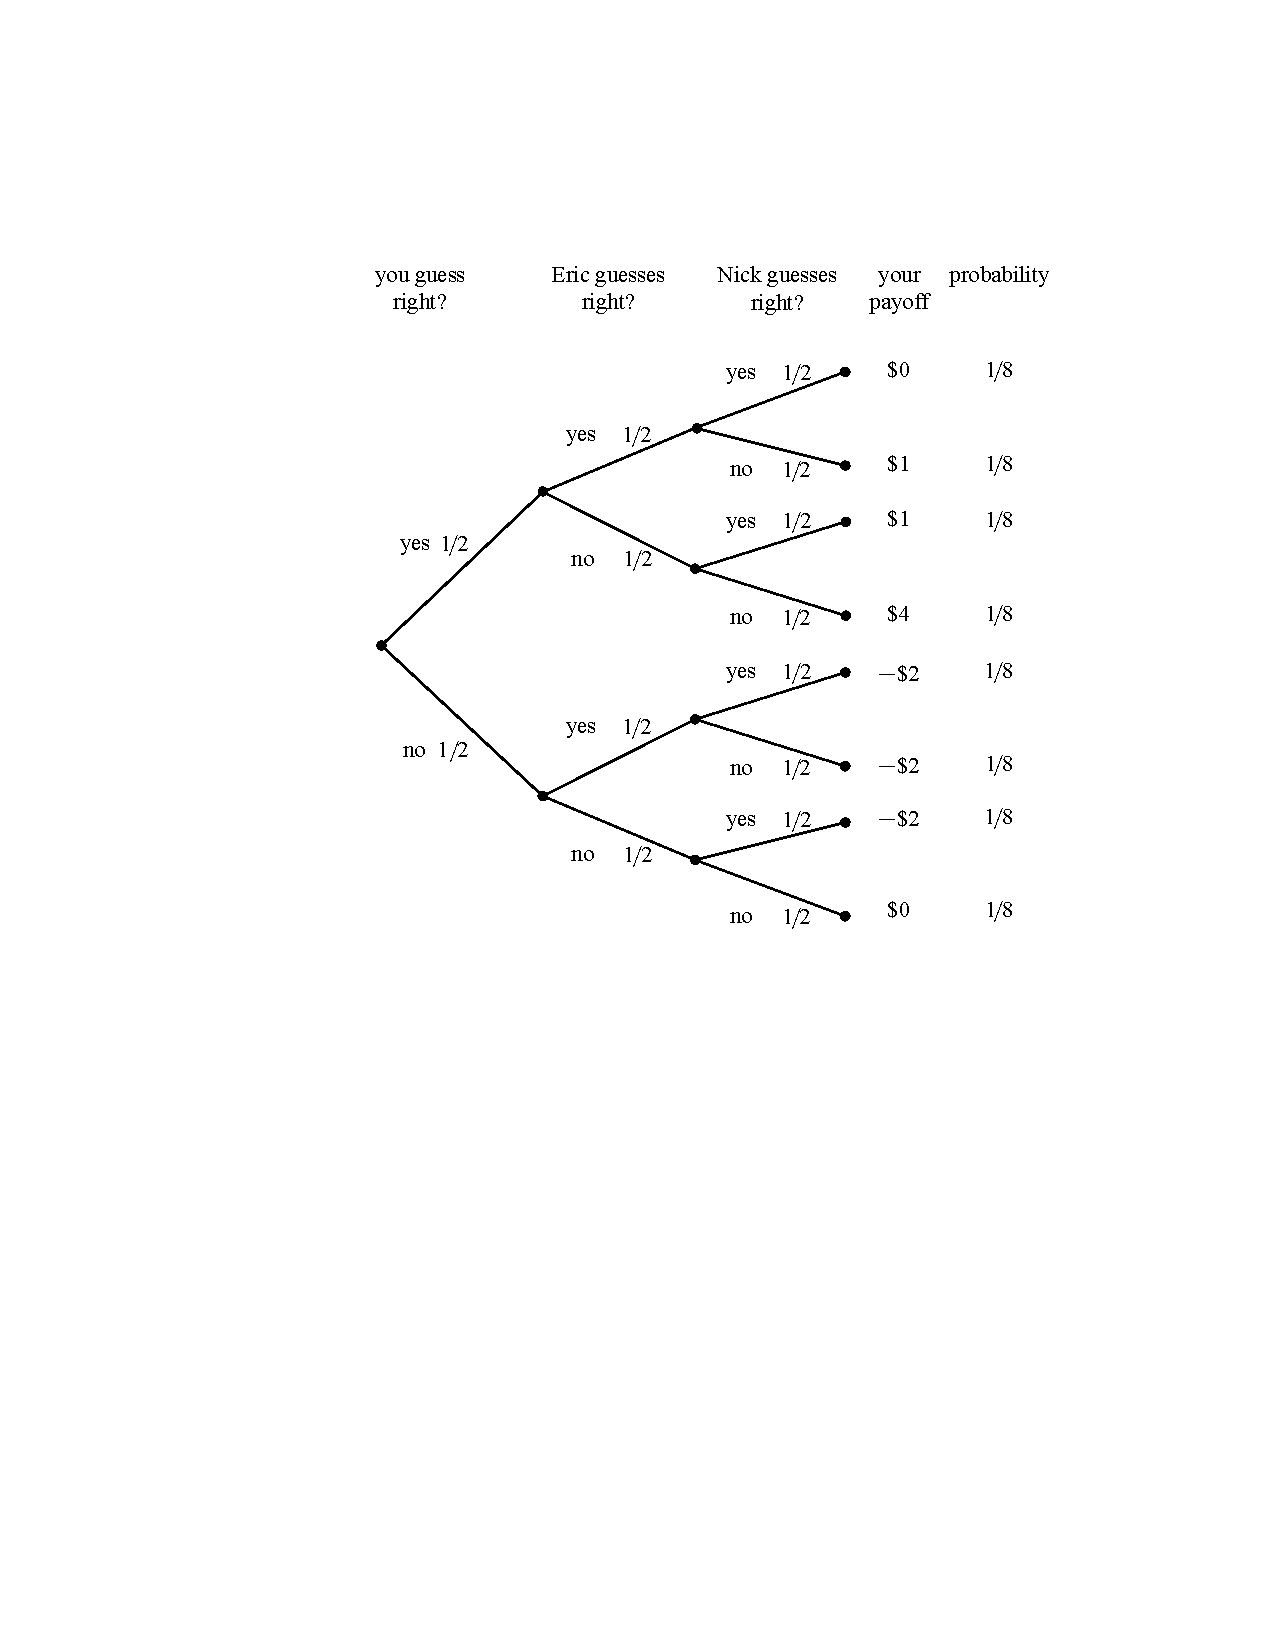
\includegraphics[width=.7\textwidth]{fig186.pdf}
	\end{block}
\end{frame}

\begin{frame}
\begin{qstn}
	\begin{itemize}
		\item<+-> Giá trị  
		\[
			\ex[\text{ Số tiền Lãi }] = ?
		\]
		\item<+-> Chuyên gì xảy ra nếu Eric và Nick luôn đặt ngược nhau?
	\end{itemize}
\end{qstn}
\end{frame}
%--- Next Frame ---%

\begin{frame}
	\begin{block}{}
\centering
	    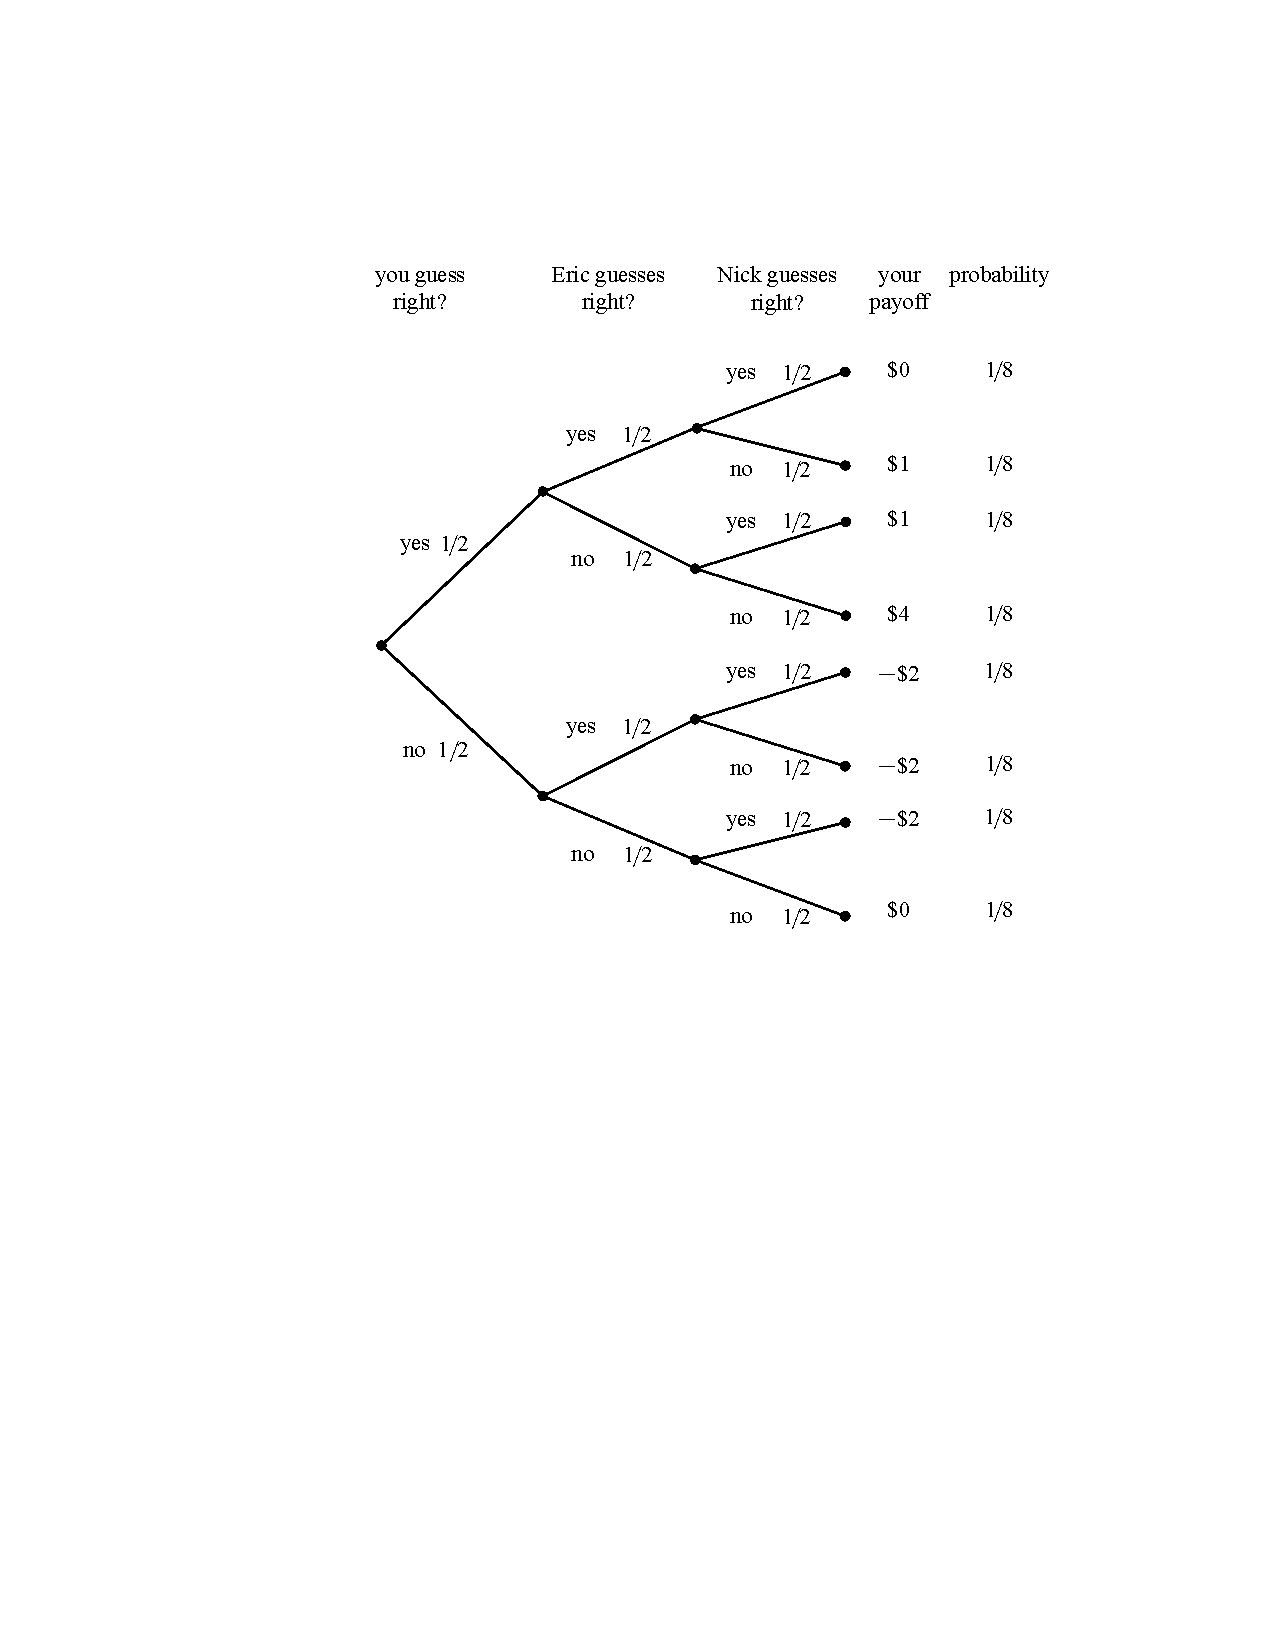
\includegraphics[width=.7\textwidth]{fig186.pdf}
	\end{block}
\end{frame}
%--- Next Frame ---%



\begin{frame}
	\begin{qstn}
		Trong trường hợp Eric và Nick luôn đặt ngược nhau thì  
		\[
			\ex[\text{ Số tiền Lãi }] = ?
		\] 
	\end{qstn}
\end{frame}
%--- Next Frame ---%


\begin{frame}{Làm thế nào để thắng xổ số?}
	\begin{itemize}
		\item Người chơi đặt $\$1$ và chọn $4$ số trong khoảng $1$ đến $36$;
		\item Công ty sổ xố của nhà nước rút ngẫu nhiên $4$ số  trong khoảng $1$ đến~$36$;
		\item Công ty sổ xố chia đều $1/2$ số tiền thu được cho  những người đoán đúng
và dành một nửa còn lại cho ngân sách.
	\end{itemize}
\end{frame}
%--- Next Frame ---%

\begin{frame}{Khám phá của Herman Chernoff}
\begin{minipage}[c]{0.6\textwidth}
	Phần lớn mọi người chọn số giống nhau. Có vẻ như họ nghĩ theo cũng một cách.
	\bigskip

	Vậy, họ hợp tác với nhau để giành phần thua! Nếu họ đoán đúng, họ sẽ phải chia sẻ phần thưởng với nhiều người khác.
	\bigskip
		
	Vậy thì, chọn ngẫu nhiên là một lợi thế. Kỳ vọng Lãi  là $+\$0.7$ chứ không phải là $-\$0.5$.
\end{minipage}\qquad 
	\begin{minipage}[c]{0.3\textwidth}
		\begin{figure}[h]
		  \centering
		    
\includegraphics[width=\textwidth]{Chernoff.pdf}
		\end{figure}
		
	\end{minipage}
\end{frame}
%--- Next Frame ---%
\begin{frame}{Định nghĩa tương đương của kỳ vọng}
	\begin{thrm}
		$$\ex[R] = \sum_{x \in Range(R)} x \cdot \pr[R = x].$$
	\end{thrm}
	\vspace{-0.5cm}
	
	\action<2->{	\begin{align*}
			\ex[R] &=  \sum_{w \in \mathcal{S}} R(w)\pr[w] \\
			       \action<3->{&=  \sum_{x \in Range(R)}\ \sum_{w \in [R=x]} R(w)\pr[w] \\}
			       \action<4->{&=  \sum_{x \in Range(R)}\ \sum_{w \in [R=x]} x\cdot \pr[w] \\}
			\action<5->{	   &= \sum_{x \in Range(R)}\ x \left(\sum_{w \in [R=x]} \pr[w]\right)  }
			\action<6->{	   = \sum_{x \in Range(R)} x \cdot \pr[R = x].}
		\end{align*}}
\end{frame}
%--- Next Frame ---%

\begin{frame}
	\begin{crllr}
		Nếu $R: \mathcal{S} \longrightarrow \mathbb{N}$ thì
		\[
			\ex[R] = \sum_{i=0}^{\infty} i\cdot \pr[R=i]. 
		\]
	\end{crllr}
\end{frame}
%--- Next Frame ---%

\begin{frame}
	\begin{thrm}
		Nếu $R: \mathcal{S} \longrightarrow \mathbb{N}$ thì
		\[
			\ex[R] = \sum_{i=0}^{\infty} \pr[R>i]. 
		\]		
	\end{thrm}
	\begin{proof}
	\begin{tabular}{ccr}
	$\pr[R>0]$ &$=$ &$\pr[R=1] + \pr[R=2] + \pr[R=3] + \cdots$ \\
	$\pr[R>1]$ &$=$ &           $\pr[R=2] + \pr[R=3] + \cdots$ \\
	$\pr[R>2]$ &$=$ &                      $\pr[R=3] + \cdots$ \\
	           &$\vdots$ &  \\
	\hline\\
	$\sum_{i=0}^{\infty} \pr[R>i]$ &$=$ &$\sum_{i=0}^{\infty} i\cdot\pr[R=i]\hfill\hfill$
	\end{tabular}	
		
	\end{proof}
\end{frame}
%--- Next Frame ---%

\begin{frame}
	\begin{qstn}
		Xét một hệ thống chạy với xác suất xảy ra lỗi (độc lập) tại mỗi bước là~$p$.  
		\[
			R = \text{ bước  xuất hiện lỗi }.
		\]  
		Hãy tính $\ex[R]$.
	\end{qstn}
\end{frame}
%--- Next Frame ---%

\begin{frame}
	\begin{sol}
		\begin{align*}
			\action<+->{\ex[R] &= \sum_{i=0}^{\infty} i\cdot \pr[R = i]} \action<+->{= \sum_{i=0}^{\infty} \overbrace{\pr[R > i]}^{{\color{blue!60}\pr[ \text{ $i$ bước đầu OK  }]}} \\}
			\action<+->{&=\sum_{i=0}^{\infty} \pr[\text{ OK bước 1 }]\cdot \pr[\text{ OK bước 2 }] \cdots\pr[\text{ OK bước $i$ }  ] \\}
			\action<+->{&= \sum_{i=0}^{\infty} (1- p)^i\\}
			\action<+->{&= \frac{1}{1 - (1-p)}\\}
			\action<+->{& = 1/p}
		\end{align*}
	\end{sol}
\end{frame}

\begin{frame}
	\begin{qstn}
		Về trung bình, cần sinh bao nhiêu lần thì có được con gái biết rằng $\pr[ \text{ sinh con gái }] = 1/2$?
	\end{qstn}
\end{frame}

%--- Next Frame ---%
\begin{frame}
	\begin{qstn}
		Xét $D$ là thời gian trễ của gói tin. Nếu 
		\[
			\pr[D>i] = 1/i
		\]
		thì thời gian trễ trung bình của gói tin bằng bao nhiêu?
	\end{qstn}
\action<2->{		\begin{align*}
			\ex[D] &= \sum_{i=1}^{\infty} \pr[D\geq i] \\
			       \action<3->{&= \sum_{i=1}^{\infty} 1/i}\action<4->{ = \infty.}
		\end{align*}
}
\end{frame}
%--- Next Frame ---%

\begin{frame}{Tính tuyến tính của kỳ vọng}
	\begin{thrm}
		Với các biến ngẫu nhiên $R_1,R_2$ (không nhất thiết phải độc lập) trên không gian xác suất $\mathcal{S}$,
		\[
			\ex[R_1 + R_2] = \ex[R_1] + \ex[R_2].
		\]
	\end{thrm}
\end{frame}
%--- Next Frame ---%

\begin{frame}{Tính tuyến tính của kỳ vọng}
	\begin{crllr}
		Với các biến ngẫu nhiên $R_1,R_2,\dots, R_n$ (không nhất thiết phải độc lập) trên không gian xác suất $\mathcal{S}$,
		\[
			\ex[R_1 + R_2 + \cdots + R_n] = \ex[R_1] + \ex[R_2] + \cdots + \ex[R_n].
		\]
	\end{crllr}
	
\end{frame}
%--- Next Frame ---%

\begin{frame}
	\begin{xmpl}
		Tung hai con xúc xắc và đặt 
		\begin{align*}
			R_1 = \text{ kết quả của con xúc xắc } 1 \\
			R_2 = \text{ kết quả của con xúc xắc } 2 			
		\end{align*}
		Vậy thì 
		\begin{align*}
				\ex[R_1 + R_2] \action<2->{&= \ex[R_1] + \ex[R_2]\\}
				               \action<3->{&= 3.5 + 3.5 = 7.}
		\end{align*}
	\end{xmpl}
\end{frame}
%--- Next Frame ---%

\begin{frame}
	\begin{block}{Bài toán kiểm tra mũ}
		Có $n$ người đàn ông đến Casino. Mỗi người có một cái mũ. Khi đến, họ cất mũ lên giá.  Khi về, mỗi người lấy ngẫu nhiên một chiếc mũ. Đặt 
		\[
			R = \text{ Số người lấy đúng mũ của mình. }
		\] 
		Hãy tính $\ex[R]$.
	\end{block}
\action<2->{	\begin{align*}
		\ex[R] &= \sum_{i=0}^n k\cdot \pr[R = k] \\
		\pr[R=k] &= \begin{cases}
			\frac{1}{k!(n-k)!} & \text{ với } k \leq n-2 \\
			0 & \text{ với } k = n-1 \\
			\frac{1}{n!} & \text{ với } k =  n 
		\end{cases} \qquad (\text{\color{red}Sai})
	\end{align*}}
\action<3->{	Bài toán có vẻ khó!}
\end{frame}
%--- Next Frame ---%
%--- Next Frame ---%
\begin{frame}
	\begin{block}{Một lời giải dễ}
	Đặt 
	\[
		R_i = \begin{cases}
			1 & \text{ nếu người thứ $i$ lấy đúng mũ } \\
			0 & \text{ ngược lại }
		\end{cases}
	\]
	\action<2->{Ta có 
	\[
		R = R_1 + R_2 + \cdots + R_n. 
	\]}
	\action<3->{Vậy thì
	\begin{align*}
		\ex[R] &= \ex[R_1] + \ex[R_2] + \dots + \ex[R_n] \\		
		       \action<4->{&= \pr[R_1 = 1] + \pr[R_2 = 1] + \cdots + \pr[R_n = 1] \\}
			\action<5->{   &= 1/n + 1/n + \cdots + 1/n \\}
			\action<6->{   &= 1.}
	\end{align*}}		
	\end{block}
\end{frame}
%--- Next Frame ---%

\begin{frame}{Bài tập}
  \begin{itemize}
  \item Một con khỉ đánh máy với  bàn phím chỉ có $26$ chữ cái thường.
  \item Mỗi ký tự được chọn độc lập và theo phân phối đều trên bảng chữ.
  \item Nếu con khỉ đánh $1,000,000$ ký tự, vậy trung bình có bao nhiêu xâu ``proof'' xuất hiện?
  \end{itemize}
\end{frame}
\end{document}



%%% Local Variables:
%%% mode: latex
%%% TeX-master: t
%%% End:
